\chapter{Algoritmos gulosos}

\index{algoritmo guloso}

Um \key{algoritmo guloso}
constrói uma solução para o problema
sempre fazendo a escolha que parece
ser a melhor no momento.
Um algoritmo guloso nunca volta atrás
em suas escolhas, mas constrói diretamente
a solução final.
Por esta razão, os algoritmos gulosos
são geralmente muito eficientes.

A dificuldade em projetar algoritmos gulosos
está em encontrar uma estratégia gulosa
que sempre produza uma solução ótima
para o problema.
As escolhas localmente ótimas num algoritmo guloso
devem ser também globalmente ótimas.
Muitas vezes é difícil argumentar que
um algoritmo guloso funciona.

\section{Problema das moedas}

Como primeiro exemplo, consideramos um problema
onde nos é dado um conjunto de moedas
e nossa tarefa é formar uma soma de dinheiro $n$
usando as moedas.
Os valores das moedas são
$\texttt{moedas}=\{c_1,c_2,\ldots,c_k\}$,
e cada moeda pode ser usada quantas vezes quisermos.
Qual é o número mínimo de moedas necessárias?

Por exemplo, se as moedas forem as moedas de euro (em centavos)
\[\{1,2,5,10,20,50,100,200\}\]
e $n=520$,
precisamos de pelo menos quatro moedas.
A solução ótima é selecionar as moedas
$200+200+100+20$ cuja soma é 520.

\subsubsection{Algoritmo guloso}

Um algoritmo guloso simples para o problema
seleciona sempre a maior moeda possível,
até que a soma de dinheiro necessária seja construída.
Este algoritmo funciona no caso de exemplo,
porque primeiro selecionamos duas moedas de 200 centavos,
depois uma moeda de 100 centavos e finalmente uma moeda de 20 centavos.
Mas será que este algoritmo funciona sempre?

Acontece que se as moedas são as moedas de euro,
o algoritmo guloso \emph{sempre} funciona, i.e.,
ele produz sempre uma solução com o menor número
possível de moedas.
A correção do algoritmo pode ser
mostrada da seguinte forma:

Primeiro, cada moeda de 1, 5, 10, 50 e 100 aparece
no máximo uma vez numa solução ótima,
porque se a
solução contivesse duas moedas dessas,
poderíamos substituí-las por uma moeda e
obter uma solução melhor.
Por exemplo, se a solução contivesse
as moedas $5+5$, poderíamos substituí-las pela moeda $10$.

Da mesma forma, as moedas de 2 e 20 aparecem
no máximo duas vezes numa solução ótima,
porque poderíamos substituir
as moedas $2+2+2$ pelas moedas $5+1$ e
as moedas $20+20+20$ pelas moedas $50+10$.
Além disso, uma solução ótima não pode conter
as moedas $2+2+1$ ou $20+20+10$,
porque poderíamos substituí-las pelas moedas $5$ e $50$.

Usando estas observações,
podemos mostrar para cada moeda $x$ que
não é possível construir de forma ótima
uma soma $x$ ou qualquer soma maior usando apenas moedas
que são menores que $x$.
Por exemplo, se $x=100$, a maior soma ótima
usando as moedas menores é $50+20+20+5+2+2=99$.
Assim, o algoritmo guloso que seleciona sempre
a maior moeda produz a solução ótima.

Este exemplo mostra que pode ser difícil
argumentar que um algoritmo guloso funciona,
mesmo que o próprio algoritmo seja simples.

\subsubsection{Caso geral}

No caso geral, o conjunto de moedas pode conter quaisquer moedas
e o algoritmo guloso \emph{não} produz necessariamente
uma solução ótima.

Podemos provar que um algoritmo guloso não funciona
mostrando um contraexemplo
onde o algoritmo dá uma resposta errada.
Neste problema podemos facilmente encontrar um contraexemplo:
se as moedas são $\{1,3,4\}$ e a soma alvo
é 6, o algoritmo guloso produz a solução
$4+1+1$ enquanto que a solução ótima é $3+3$.

Não se sabe se o problema geral das moedas
pode ser resolvido usando algum algoritmo guloso\footnote{No entanto, é possível
\emph{verificar} em tempo polinomial
se o algoritmo guloso apresentado neste capítulo funciona para
um dado conjunto de moedas \cite{pea05}.}.
No entanto, como veremos no Capítulo 7,
em alguns casos,
o problema geral pode ser eficientemente
resolvido usando um algoritmo de
programação dinâmica que dá sempre a resposta correta.

\section{Escalonamento}

Muitos problemas de escalonamento podem ser resolvidos
usando algoritmos gulosos.
Um problema clássico é o seguinte:
Dados $n$ eventos com seus horários de início e fim,
encontre um escalonamento
que inclua o maior número possível de eventos.
Não é possível selecionar um evento parcialmente.
Por exemplo, considere os seguintes eventos:
\begin{center}
\begin{tabular}{lll}
evento & hora de início & hora de fim \\
\hline
$A$ & 1 & 3 \\
$B$ & 2 & 5 \\
$C$ & 3 & 9 \\
$D$ & 6 & 8 \\
\end{tabular}
\end{center}
Neste caso, o número máximo de eventos é dois.
Por exemplo, podemos selecionar os eventos $B$ e $D$
da seguinte forma:
\begin{center}
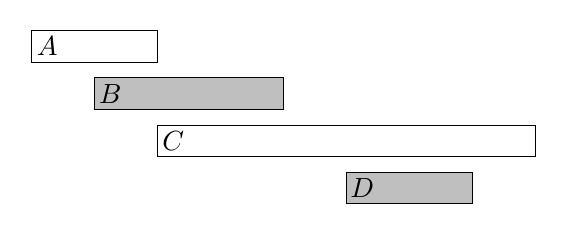
\begin{tikzpicture}[scale=.4]
  \begin{scope}
    \draw (2, 0) rectangle (6, -1);
    \draw[fill=lightgray] (4, -1.5) rectangle (10, -2.5);
    \draw (6, -3) rectangle (18, -4);
    \draw[fill=lightgray] (12, -4.5) rectangle (16, -5.5);
    \node at (2.5,-0.5) {$A$};
    \node at (4.5,-2) {$B$};
    \node at (6.5,-3.5) {$C$};
    \node at (12.5,-5) {$D$};
  \end{scope}
\end{tikzpicture}
\end{center}

É possível inventar vários algoritmos gulosos
para o problema, mas qual deles funciona em todos os casos?

\subsubsection*{Algoritmo 1}

A primeira ideia é selecionar os eventos
\emph{mais curtos} possíveis.
No caso de exemplo, este algoritmo
seleciona os seguintes eventos:
\begin{center}
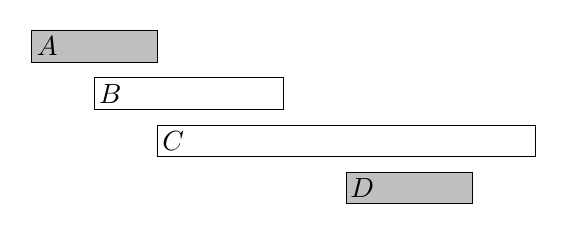
\begin{tikzpicture}[scale=.4]
  \begin{scope}
    \draw[fill=lightgray] (2, 0) rectangle (6, -1);
    \draw (4, -1.5) rectangle (10, -2.5);
    \draw (6, -3) rectangle (18, -4);
    \draw[fill=lightgray] (12, -4.5) rectangle (16, -5.5);
    \node at (2.5,-0.5) {$A$};
    \node at (4.5,-2) {$B$};
    \node at (6.5,-3.5) {$C$};
    \node at (12.5,-5) {$D$};
  \end{scope}
\end{tikzpicture}
\end{center}

No entanto, selecionar eventos curtos nem sempre
é uma estratégia correta. Por exemplo, o algoritmo falha
no seguinte caso:
\begin{center}
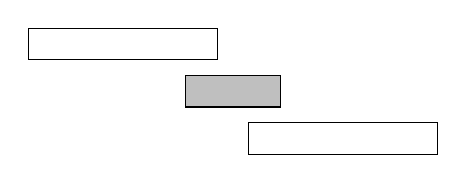
\begin{tikzpicture}[scale=.4]
  \begin{scope}
    \draw (1, 0) rectangle (7, -1);
    \draw[fill=lightgray] (6, -1.5) rectangle (9, -2.5);
    \draw (8, -3) rectangle (14, -4);
  \end{scope}
\end{tikzpicture}
\end{center}
Se selecionarmos o evento curto, só podemos selecionar um evento.
No entanto, seria possível selecionar ambos os eventos longos.

\subsubsection*{Algoritmo 2}

Outra ideia é selecionar sempre o próximo evento possível
que \emph{começa} o mais \emph{cedo} possível.
Este algoritmo seleciona os seguintes eventos:
\begin{center}
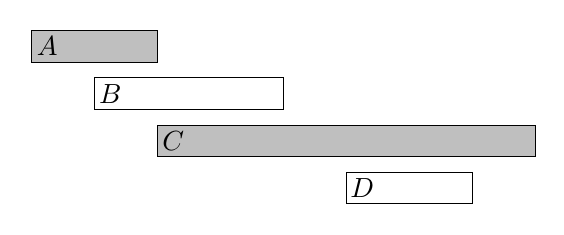
\begin{tikzpicture}[scale=.4]
  \begin{scope}
    \draw[fill=lightgray] (2, 0) rectangle (6, -1);
    \draw (4, -1.5) rectangle (10, -2.5);
    \draw[fill=lightgray] (6, -3) rectangle (18, -4);
    \draw (12, -4.5) rectangle (16, -5.5);
    \node at (2.5,-0.5) {$A$};
    \node at (4.5,-2) {$B$};
    \node at (6.5,-3.5) {$C$};
    \node at (12.5,-5) {$D$};
  \end{scope}
\end{tikzpicture}
\end{center}

No entanto, podemos encontrar um contraexemplo
também para este algoritmo.
Por exemplo, no seguinte caso,
o algoritmo seleciona apenas um evento:
\begin{center}
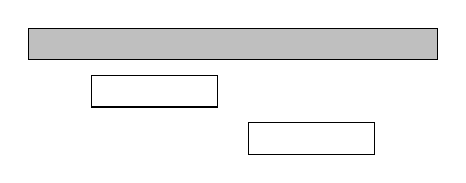
\begin{tikzpicture}[scale=.4]
  \begin{scope}
    \draw[fill=lightgray] (1, 0) rectangle (14, -1);
    \draw (3, -1.5) rectangle (7, -2.5);
    \draw (8, -3) rectangle (12, -4);
  \end{scope}
\end{tikzpicture}
\end{center}
Se selecionarmos o primeiro evento, não é possível
selecionar quaisquer outros eventos.
No entanto, seria possível selecionar os
outros dois eventos.

\subsubsection*{Algoritmo 3}

A terceira ideia é selecionar sempre o próximo
evento possível que \emph{termina} o mais \emph{cedo} possível.
Este algoritmo seleciona os seguintes eventos:
\begin{center}
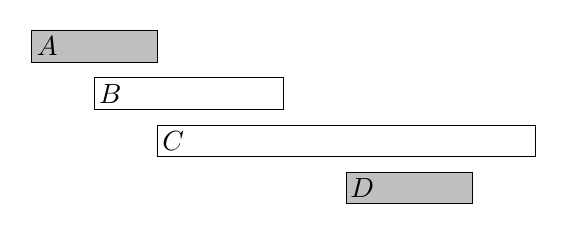
\begin{tikzpicture}[scale=.4]
  \begin{scope}
    \draw[fill=lightgray] (2, 0) rectangle (6, -1);
    \draw (4, -1.5) rectangle (10, -2.5);
    \draw (6, -3) rectangle (18, -4);
    \draw[fill=lightgray] (12, -4.5) rectangle (16, -5.5);
    \node at (2.5,-0.5) {$A$};
    \node at (4.5,-2) {$B$};
    \node at (6.5,-3.5) {$C$};
    \node at (12.5,-5) {$D$};
  \end{scope}
\end{tikzpicture}
\end{center}

Acontece que este algoritmo
\emph{sempre} produz uma solução ótima.
A razão para isso é que é sempre uma escolha ótima
selecionar primeiro um evento que termina
o mais cedo possível.
Depois disso, é uma escolha ótima
selecionar o próximo evento
usando a mesma estratégia, etc.,
até não podermos selecionar mais eventos.

Uma forma de argumentar que o algoritmo funciona
é considerar
o que acontece se selecionarmos primeiro um evento
que termina mais tarde do que o evento que termina
o mais cedo possível.
Agora, teremos no máximo um número igual de
escolhas para selecionar o próximo evento.
Portanto, selecionar um evento que termina mais tarde
nunca pode resultar numa solução melhor,
e o algoritmo guloso está correto.

\section{Tarefas e prazos}

Vamos agora considerar um problema onde
nos são dadas $n$ tarefas com durações e prazos
e nossa tarefa é escolher uma ordem para realizar as tarefas.
Para cada tarefa, ganhamos $d-x$ pontos
onde $d$ é o prazo da tarefa
e $x$ é o momento em que terminamos a tarefa.
Qual é a maior pontuação total possível
que podemos obter?

Por exemplo, suponha que as tarefas são as seguintes:
\begin{center}
\begin{tabular}{lll}
tarefa & duração & prazo \\
\hline
$A$ & 4 & 2 \\
$B$ & 3 & 5 \\
$C$ & 2 & 7 \\
$D$ & 4 & 5 \\
\end{tabular}
\end{center}
Neste caso, um escalonamento ótimo para as tarefas
é o seguinte:
\begin{center}
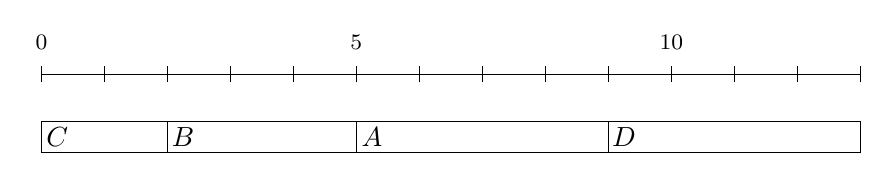
\begin{tikzpicture}[scale=.4]
  \begin{scope}
    \draw (0, 0) rectangle (4, -1);
    \draw (4, 0) rectangle (10, -1);
    \draw (10, 0) rectangle (18, -1);
    \draw (18, 0) rectangle (26, -1);
    \node at (0.5,-0.5) {$C$};
    \node at (4.5,-0.5) {$B$};
    \node at (10.5,-0.5) {$A$};
    \node at (18.5,-0.5) {$D$};

    \draw (0,1.5) -- (26,1.5);
    \foreach \i in {0,2,...,26}
    {
        \draw (\i,1.25) -- (\i,1.75);
    }
    \footnotesize
    \node at (0,2.5) {0};
    \node at (10,2.5) {5};
    \node at (20,2.5) {10};

  \end{scope}
\end{tikzpicture}
\end{center}
Nesta solução, $C$ rende 5 pontos,
$B$ rende 0 pontos, $A$ rende $-7$ pontos
e $D$ rende $-8$ pontos,
então a pontuação total é $-10$.

Surpreendentemente, a solução ótima para o problema
sequer depende dos prazos, uma estratégia gulosa 
correta é simplesmente
executar as tarefas \emph{ordenadas por suas durações}
em ordem crescente.
A razão para isso é que se alguma vez executarmos
duas tarefas, uma após a outra, de tal forma que a primeira tarefa
demore mais tempo do que a segunda tarefa,
podemos obter uma solução melhor se trocarmos as tarefas.
Por exemplo, considere o seguinte escalonamento:
\begin{center}
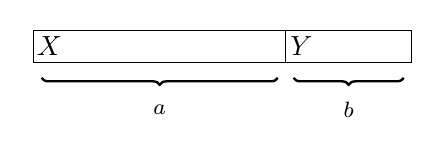
\begin{tikzpicture}[scale=.4]
  \begin{scope}
    \draw (0, 0) rectangle (8, -1);
    \draw (8, 0) rectangle (12, -1);
    \node at (0.5,-0.5) {$X$};
    \node at (8.5,-0.5) {$Y$};

\draw [decoration={brace}, decorate, line width=0.3mm] (7.75,-1.5) -- (0.25,-1.5);
\draw [decoration={brace}, decorate, line width=0.3mm] (11.75,-1.5) -- (8.25,-1.5);

\footnotesize
\node at (4,-2.5) {$a$};
\node at (10,-2.5) {$b$};

  \end{scope}
\end{tikzpicture}
\end{center}
Aqui $a>b$, então devemos trocar as tarefas:
\begin{center}
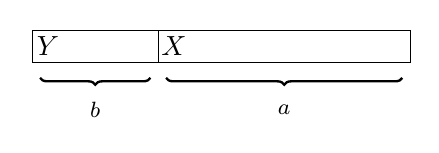
\begin{tikzpicture}[scale=.4]
  \begin{scope}
    \draw (0, 0) rectangle (4, -1);
    \draw (4, 0) rectangle (12, -1);
    \node at (0.5,-0.5) {$Y$};
    \node at (4.5,-0.5) {$X$};

\draw [decoration={brace}, decorate, line width=0.3mm] (3.75,-1.5) -- (0.25,-1.5);
\draw [decoration={brace}, decorate, line width=0.3mm] (11.75,-1.5) -- (4.25,-1.5);

\footnotesize
\node at (2,-2.5) {$b$};
\node at (8,-2.5) {$a$};

  \end{scope}
\end{tikzpicture}
\end{center}
Agora $X$ dá $b$ pontos a menos e $Y$ dá $a$ pontos a mais,
então a pontuação total aumenta em $a-b > 0$.
Numa solução ótima,
para quaisquer duas tarefas consecutivas,
deve verificar-se que a tarefa mais curta vem
antes da tarefa mais longa.
Assim, as tarefas devem ser executadas
ordenadas pelas suas durações.

\section{Minimizando somas}

Consideramos agora um problema onde
nos são dados $n$ números $a_1,a_2,\ldots,a_n$
e nossa tarefa é encontrar um valor $x$
que minimize a soma
\[|a_1-x|^c+|a_2-x|^c+\cdots+|a_n-x|^c.\]
Vamos focar nos casos $c=1$ e $c=2$.

\subsubsection{Caso $c=1$}

Neste caso, devemos minimizar a soma
\[|a_1-x|+|a_2-x|+\cdots+|a_n-x|.\]
Por exemplo, se os números são $[1,2,9,2,6]$,
a melhor solução é selecionar $x=2$
o que produz a soma
\[
|1-2|+|2-2|+|9-2|+|2-2|+|6-2|=12.
\]
No caso geral, a melhor escolha para $x$
é a \textit{mediana} dos números,
i.e., o número do meio após a ordenação.
Por exemplo, a lista $[1,2,9,2,6]$
torna-se $[1,2,2,6,9]$ após a ordenação,
então a mediana é 2.

A mediana é uma escolha ótima,
porque se $x$ é menor que a mediana,
a soma torna-se menor ao aumentar $x$,
e se $x$ é maior que a mediana,
a soma torna-se menor ao diminuir $x$.
Portanto, a solução ótima é que $x$
seja a mediana.
Se $n$ é par e existem duas medianas,
ambas as medianas e todos os valores entre elas
são escolhas ótimas.

\subsubsection{Caso $c=2$}

Neste caso, devemos minimizar a soma
\[(a_1-x)^2+(a_2-x)^2+\cdots+(a_n-x)^2.\]
Por exemplo, se os números são $[1,2,9,2,6]$,
a melhor solução é selecionar $x=4$
o que produz a soma
\[
(1-4)^2+(2-4)^2+(9-4)^2+(2-4)^2+(6-4)^2=46.
\]
No caso geral, a melhor escolha para $x$
é a \emph{média} dos números.
No exemplo, a média é $(1+2+9+2+6)/5=4$.
Este resultado pode ser derivado apresentando
a soma da seguinte forma:
\[
nx^2 - 2x(a_1+a_2+\cdots+a_n) + (a_1^2+a_2^2+\cdots+a_n^2)
\]
A última parte não depende de $x$,
portanto podemos ignorá-la.
As partes restantes formam uma função
$nx^2-2xs$ onde $s=a_1+a_2+\cdots+a_n$.
Esta é uma parábola com a concavidade voltada para cima
com raízes $x=0$ e $x=2s/n$,
e o valor mínimo é a média
das raízes $x=s/n$, i.e.,
a média dos números $a_1,a_2,\ldots,a_n$.

\section{Compressão de dados}

\index{compressão de dados}
\index{código binário}
\index{palavra de código}

Um \key{código binário} atribui para cada caractere
de uma string uma \key{palavra de código} que consiste em bits.
Podemos \emph{comprimir} a string usando o código binário
substituindo cada caractere pela
palavra de código correspondente.
Por exemplo, o seguinte código binário
atribui palavras de código para os caracteres
\texttt{A}–\texttt{D}:
\begin{center}
\begin{tabular}{rr}
caractere & palavra de código \\
\hline
\texttt{A} & 00 \\
\texttt{B} & 01 \\
\texttt{C} & 10 \\
\texttt{D} & 11 \\
\end{tabular}
\end{center}
Este é um código de \key{comprimento constante}
o que significa que o comprimento de cada
palavra de código é o mesmo.
Por exemplo, podemos comprimir a string
\texttt{AABACDACA} da seguinte forma:
\[00\,00\,01\,00\,10\,11\,00\,10\,00\]
Usando este código, o comprimento da string comprimida
é de 18 bits.
No entanto, podemos comprimir a string melhor
se usarmos um código de \key{comprimento variável}
onde as palavras de código podem ter comprimentos diferentes.
Então podemos dar palavras de código curtas para
caracteres que aparecem frequentemente
e palavras de código longas para caracteres
que aparecem raramente.
Acontece que um código \key{ótimo}
para a string acima é o seguinte:
\begin{center}
\begin{tabular}{rr}
caractere & palavra de código \\
\hline
\texttt{A} & 0 \\
\texttt{B} & 110 \\
\texttt{C} & 10 \\
\texttt{D} & 111 \\
\end{tabular}
\end{center}
Um código ótimo produz uma string comprimida
que é o mais curta possível.
Neste caso, a string comprimida usando
o código ótimo é
\[0\,0\,110\,0\,10\,111\,0\,10\,0,\]
então são necessários apenas 15 bits em vez de 18 bits.
Assim, graças a um código melhor, foi possível
poupar 3 bits na string comprimida.

Exigimos que nenhuma palavra de código
seja um prefixo de outra palavra de código.
Por exemplo, não é permitido que um código
contenha ambas as palavras de código 10
e 1011.
A razão para isso é que queremos
ser capazes de gerar a string original
a partir da string comprimida.
Se uma palavra de código pudesse ser um prefixo de outra palavra de código,
isso nem sempre seria possível.
Por exemplo, o seguinte código \emph{não} é válido:
\begin{center}
\begin{tabular}{rr}
caractere & palavra de código \\
\hline
\texttt{A} & 10 \\
\texttt{B} & 11 \\
\texttt{C} & 1011 \\
\texttt{D} & 111 \\
\end{tabular}
\end{center}
Usando este código, não seria possível saber
se a string comprimida 1011 corresponde à
string \texttt{AB} ou à string \texttt{C}.

\index{Codificação de Huffman}

\subsubsection{Codificação de Huffman}

\key{Codificação de Huffman}\footnote{D. A. Huffman descobriu este método
ao resolver um trabalho de um curso universitário
e publicou o algoritmo em 1952 \cite{huf52}.} é um algoritmo guloso
que constrói um código ótimo para
comprimir uma dada string.
O algoritmo constrói uma árvore binária
com base nas frequências dos caracteres
na string,
e a palavra de código de cada caractere pode ser lida
seguindo um caminho desde a raiz até
ao nó correspondente.
Um movimento para a esquerda corresponde ao bit 0,
e um movimento para a direita corresponde ao bit 1.

Inicialmente, cada caractere da string é
representado por um nó cujo peso é o
número de vezes que o caractere ocorre na string.
Então, em cada passo, dois nós com pesos mínimos
são combinados criando
um novo nó cujo peso é a soma dos pesos
dos nós originais.
O processo continua até que todos os nós tenham sido combinados.

A seguir, veremos como a Codificação de Huffman cria
o código ótimo para a string
\texttt{AABACDACA}.
Inicialmente, existem quatro nós que correspondem
aos caracteres da string:

\begin{center}
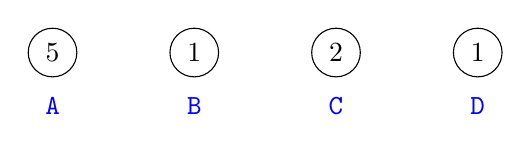
\begin{tikzpicture}[scale=0.9]
\node[draw, circle] (1) at (0,0) {$5$};
\node[draw, circle] (2) at (2,0) {$1$};
\node[draw, circle] (3) at (4,0) {$2$};
\node[draw, circle] (4) at (6,0) {$1$};

\node[color=blue] at (0,-0.75) {\texttt{A}};
\node[color=blue] at (2,-0.75) {\texttt{B}};
\node[color=blue] at (4,-0.75) {\texttt{C}};
\node[color=blue] at (6,-0.75) {\texttt{D}};

%\path[draw,thick,-] (4) -- (5);
\end{tikzpicture}
\end{center}
O nó que representa o caractere \texttt{A}
tem peso 5 porque o caractere \texttt{A}
aparece 5 vezes na string.
Os outros pesos foram calculados
da mesma forma.

O primeiro passo é combinar os nós que
correspondem aos caracteres \texttt{B} e \texttt{D},
ambos com peso 1.
O resultado é:
\begin{center}
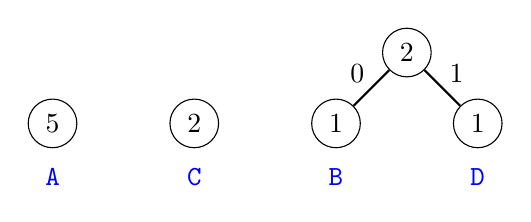
\begin{tikzpicture}[scale=0.9]
\node[draw, circle] (1) at (0,0) {$5$};
\node[draw, circle] (3) at (2,0) {$2$};
\node[draw, circle] (2) at (4,0) {$1$};
\node[draw, circle] (4) at (6,0) {$1$};
\node[draw, circle] (5) at (5,1) {$2$};

\node[color=blue] at (0,-0.75) {\texttt{A}};
\node[color=blue] at (2,-0.75) {\texttt{C}};
\node[color=blue] at (4,-0.75) {\texttt{B}};
\node[color=blue] at (6,-0.75) {\texttt{D}};

\node at (4.3,0.7) {0};
\node at (5.7,0.7) {1};

\path[draw,thick,-] (2) -- (5);
\path[draw,thick,-] (4) -- (5);
\end{tikzpicture}
\end{center}
Depois disso, os nós com peso 2 são combinados:
\begin{center}
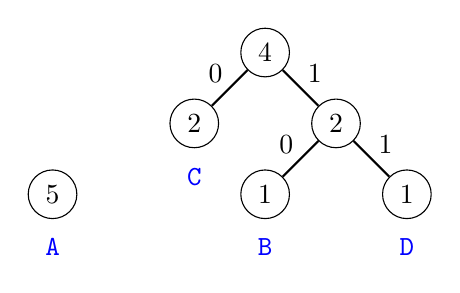
\begin{tikzpicture}[scale=0.9]
\node[draw, circle] (1) at (1,0) {$5$};
\node[draw, circle] (3) at (3,1) {$2$};
\node[draw, circle] (2) at (4,0) {$1$};
\node[draw, circle] (4) at (6,0) {$1$};
\node[draw, circle] (5) at (5,1) {$2$};
\node[draw, circle] (6) at (4,2) {$4$};

\node[color=blue] at (1,-0.75) {\texttt{A}};
\node[color=blue] at (3,1-0.75) {\texttt{C}};
\node[color=blue] at (4,-0.75) {\texttt{B}};
\node[color=blue] at (6,-0.75) {\texttt{D}};

\node at (4.3,0.7) {0};
\node at (5.7,0.7) {1};
\node at (3.3,1.7) {0};
\node at (4.7,1.7) {1};

\path[draw,thick,-] (2) -- (5);
\path[draw,thick,-] (4) -- (5);
\path[draw,thick,-] (3) -- (6);
\path[draw,thick,-] (5) -- (6);
\end{tikzpicture}
\end{center}
Finalmente, os dois nós restantes são combinados:
\begin{center}
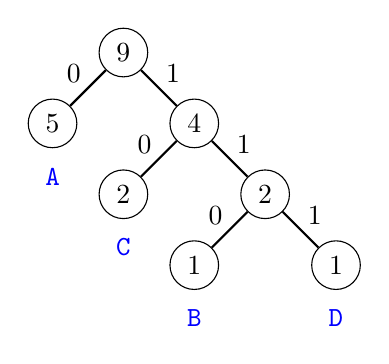
\begin{tikzpicture}[scale=0.9]
\node[draw, circle] (1) at (2,2) {$5$};
\node[draw, circle] (3) at (3,1) {$2$};
\node[draw, circle] (2) at (4,0) {$1$};
\node[draw, circle] (4) at (6,0) {$1$};
\node[draw, circle] (5) at (5,1) {$2$};
\node[draw, circle] (6) at (4,2) {$4$};
\node[draw, circle] (7) at (3,3) {$9$};

\node[color=blue] at (2,2-0.75) {\texttt{A}};
\node[color=blue] at (3,1-0.75) {\texttt{C}};
\node[color=blue] at (4,-0.75) {\texttt{B}};
\node[color=blue] at (6,-0.75) {\texttt{D}};

\node at (4.3,0.7) {0};
\node at (5.7,0.7) {1};
\node at (3.3,1.7) {0};
\node at (4.7,1.7) {1};
\node at (2.3,2.7) {0};
\node at (3.7,2.7) {1};

\path[draw,thick,-] (2) -- (5);
\path[draw,thick,-] (4) -- (5);
\path[draw,thick,-] (3) -- (6);
\path[draw,thick,-] (5) -- (6);
\path[draw,thick,-] (1) -- (7);
\path[draw,thick,-] (6) -- (7);
\end{tikzpicture}
\end{center}

Agora todos os nós estão na árvore, então o código está pronto.
As seguintes palavras de código podem ser lidas a partir da árvore:
\begin{center}
\begin{tabular}{rr}
caractere & palavra de código \\
\hline
\texttt{A} & 0 \\
\texttt{B} & 110 \\
\texttt{C} & 10 \\
\texttt{D} & 111 \\
\end{tabular}
\end{center}
